\section{Specifica della componente Controller}
Questa componente è incaricata di gestire la comunicazione con il client restituendo i dati richiesti o lanciando delle opportune eccezioni.
Tale componente è composta dalle classi:
\begin{itemize}
	\item \texttt{com.sirius.sequenziatore.server.controller.common.SignUpController}
	\item \texttt{com.sirius.sequenziatore.server.controller.common.LoginController}
	\item \texttt{com.sirius.sequenziatore.server.controller.common.StepInfoController}
	\item \texttt{com.sirius.sequenziatore.server.controller.common.ProcessInfoController}
	\item \texttt{com.sirius.sequenziatore.server.controller.processowner.StepController}
	\item \texttt{com.sirius.sequenziatore.server.controller.processowner.ProcessController}
	\item \texttt{com.sirius.sequenziatore.server.controller.processowner.ApproveStepController}
	\item \texttt{com.sirius.sequenziatore.server.controller.user.UserStepController}
	\item \texttt{com.sirius.sequenziatore.server.controller.user.UserProcessController}
	\item \texttt{com.sirius.sequenziatore.server.controller.user.ReportController}
\end{itemize}
Nella prossime sezioni verranno trattate in dettaglio le seguenti classi dividendo l' esposizione per \textit{package}, si evidenzia come la voce mappatura base sia l' estensione della mappatura su cui si programma il sistema che sarà \textit{localhost:8080/sequenziatore/} , quindi tutte le mappature base saranno da considerarsi come aggiunte a seguito di /sequenziatore/ e successivamente le varie varianti dei metodi.
Tutte le classi \textit{controller} dovranno essere marcate come \textit{@Controller} per essere riconosciute in modo corretto da \textit{Spring}.
\subsubsection{Package com.sirius.sequenziatore.server.controller.common}
\
\begin{figure}[H] \centering 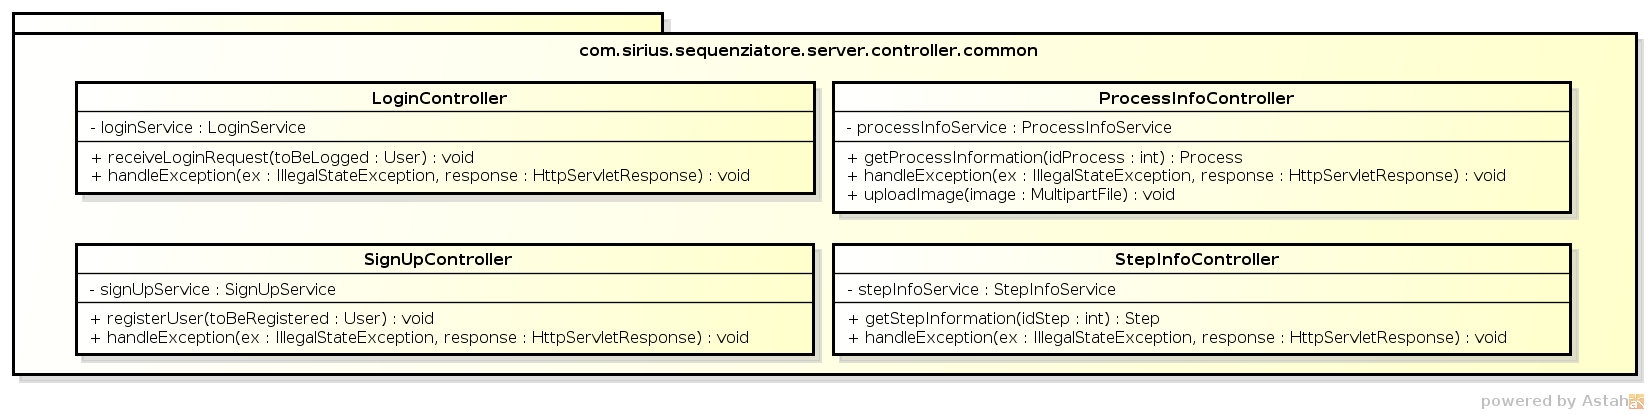
\includegraphics[width=%
\textwidth]
{./classi/server/controllercommon.png} \caption{Diagramma package - \texttt{com.sirius.sequenziatore.server.controller.common}}
\end{figure}
All' interno di questa sezione verranno trattate tutte le classi contenute nel package \textit{common}.
\paragraph{SignUpController}%--------------------------------------------------------%
\
\begin{figure}[H] \centering
\includegraphics[trim=0cm 0.8cm 0cm 0cm,clip=true,scale=0.75]%
{./classi/server/signupcontroller.png} \caption{Diagramma classe - \texttt{SignUpController}}
\end{figure}
\begin{itemize}
	\item \textbf{Descrizione: } Questa classe dovrà gestire tutte le richieste di registrazione al sistema, sarà incaricata di inserire i dati nel database e di avvertire il client della riuscita della registrazione.
	\item \textbf{Mappatura base: }\textit{\slash signup}
	\item \textbf{Relazioni con altri componenti: }
	La classe utilizzerà le seguenti classi:
	\begin{itemize}
		\item \texttt{com.sirius.sequenziatore.server.model.User;}
		\item \texttt{com.sirius.sequenziatore.server.service.SignUpService;}
	\end{itemize}
	\item \textbf{Attributi:}\begin{itemize}
					\item \texttt{-SignUpService signUpService}:\\
					oggetto di tipo com.sirius.sequenziatore.server.service.SignUpService a cui viene affidata l' elaborazione della registrazione di un utente;
	\end{itemize}
	\item \textbf{Metodi: }\begin{itemize}
					\item \texttt{+void registerUser(User toBeRegistered)}:\\
					 questo metodo gestirà una richiesta di tipo \textbf{POST} e dovrà lanciare un' eccezione di tipo \texttt{HttpError} qual' ora ci siano stati problemi nella registrazione;
					 \item \texttt{+void handleException(IllegalStateException,HttpServletResponse response)}:\\
					 questo metodo è un gestore delle eccezioni e sarà incaricato di lanciare al client un errore 409.
				\end{itemize}
\end{itemize}
\paragraph{LoginController}%--------------------------------------------------------------------%
\
\begin{figure}[H] \centering
\includegraphics[trim=0cm 0.8cm 0cm 0cm,clip=true,scale=0.75]%
{./classi/server/logincontroller.png} \caption{Diagramma classe - \texttt{LoginController}}
\end{figure}
\begin{itemize}
	\item \textbf{Descrizione: }Questa classe gestirà le richieste di \textit{log in}, delegando l' elaborazione al \textit{service} e poi avvisare il \textit{client} se l' utente è un \textit{process owner} , un utente normale o ci sono stati degli errori, in quest' ultimo caso dovrà lanciare un' eccezione;
	\item \textbf{Mappatura base: }\textit{\slash login}
	\item \textbf{Relazioni con altri componenti: }
	La classe utilizzerà le seguenti classi:
	\begin{itemize}
		\item \texttt{com.sirius.sequenziatore.server.model.User;}
		\item \texttt{com.sirius.sequenziatore.server.service.LoginService}
	\end{itemize}
	\item \textbf{Attributi: }\begin{itemize}
				\item \texttt{LoginService loginService}:\\
				oggetto di tipo com.sirius.sequenziatore.server.service.LoginService a cui viene affidata l' elaborazione della login;
	\end{itemize}
	\item \textbf{Metodi: }\begin{itemize}
					\item \texttt{+String receiveLoginRequest(User toBeLogged)}:\\
					 questo metodo gestirà un metodo di tipo \textbf{POST} , controllerà le credenziali di accesso e dovrà lanciare un' eccezione di tipo \texttt{HttpError} qualora ci siano stati problemi nella login;
					  \item \texttt{+void handleException(IllegalStateException,HttpServletResponse response)}:\\
					 questo metodo è un gestore delle eccezioni e sarà incaricato di lanciare al client un errore 422.
				\end{itemize}
\end{itemize}
\paragraph{StepInfoController}%--------------------------------------------------------------------%
\begin{figure}[H] \centering
\
\includegraphics[trim=0cm 0.8cm 0cm 0cm,clip=true,scale=0.75]%
{./classi/server/stepinfocontroller.png} \caption{Diagramma classe - \texttt{StepInfoController}}
\end{figure}
\begin{itemize}
	\item \textbf{Descrizione: }Questa classe restituirà lo scheletro, quindi la composizione del passo richiesto;
	\item \textbf{Mappatura base: }\textit{\slash step\slash \{id\}}
	\item \textbf{Relazioni con altri componenti: }
	La classe utilizzerà le seguenti classi:
	\begin{itemize}
		\item \texttt{com.sirius.sequenziatore.server.model.Step;}
		\item \texttt{com.sirius.sequenziatore.server.service.StepInfoService;}
	\end{itemize}
	\item \textbf{Metodi: }\begin{itemize}
					\item \texttt{+Step getStepInformation(int idStep)}:\\
					 il metodo gestisce una richiesta di tipo \textbf{GET} restituendo la struttura del passo con id uguale all' id fornito dopo averla richiesta al service;
					  \item \texttt{+void handleException(IllegalStateException,HttpServletResponse response)}:\\
					 questo metodo è un gestore delle eccezioni e sarà incaricato di lanciare al client un errore 404.
				\end{itemize}
\end{itemize}
\paragraph{ProcessInfoController}%----------------------------------------------------------------%
\begin{figure}[H] \centering
\includegraphics[trim=0cm 0.8cm 0cm 0cm,clip=true,scale=0.75]%
{./classi/server/processinfocontroller.png} \caption{Diagramma classe - \texttt{ProcessInfoController}}
\end{figure}
\begin{itemize}
	\item \textbf{Descrizione: } Questa classe dovrà restituire a chi lo richiede un processo dato l' \textit{id} con i suoi dati;
	\item \textbf{Mappatura base: }\textit{\slash process\slash \{id\}}
	\item \textbf{Relazioni con altri componenti: }
	La classe utilizzerà le seguenti classi:
	\begin{itemize}
		\item \texttt{com.sirius.sequenziatore.server.model.Process;}
		\item \texttt{com.sirius.sequenziatore.server.service.ProcessInfoService;}
	\end{itemize}
	\item \textbf{Metodi: }\begin{itemize}
					\item \texttt{+Process getProcessInformation(int idProcess)}:\\
					il metodo gestisce una richiesta di tipo \textbf{GET} e restituisce la struttura di un processo con l' id processo richiesto;
					 \item \texttt{+void handleException(IllegalStateException,HttpServletResponse response)}:\\
					 questo metodo è un gestore delle eccezioni e sarà incaricato di lanciare al client un errore 422.
					 \item \texttt{+boolean uploadImage(MultipartFile image)}:\\
					 il metodo gestisce una richiesta di tipo \textbf{POST} in \textit{\slash process\slash \{id\}\slash saveimage}  e affida al service l' incarico di salvare l' immagine.
				\end{itemize}
\end{itemize}